%
% Frontmatter - Introducción. Los miembros del tribunal que juzgan los PFC's tienen muchas más memorias que leer, por lo que
%	agradecerán cualquier detalle que permita facilitarles la vida. En este sentido, realizar una pequeña introducción,
%	comentar la organización y estructura de la memoria y resumir brevemente cada capítulo puede ser una buena práctica
%	que permita al lector centrarse fácilmente en la parte que más le interesa.
%

\chapter[Introducción]{Introdución}

Neste capítulo de introdución intentarase explicar os aspectos necesarios para entender en que consiste o proxecto, o que me fixo levalo a cabo e, por último, unha explicación da estrutura da presente memoria.

\section{Internacionalización e Localización de Software}
A internacionalización é o proceso de adaptación dun software para que este poida ser traducido a varios idiomas e ser usado en diferentes rexións sen modificar a súa enxeñería. A localización de software consiste na adaptación de dito software a unha rexión determinada. Isto aínda que afecta fundamentalmente ó idioma, tamén ten outros elementos como as divisas, a forma de formatar as datas ou símbolos que nunhas áreas teñen un significado e noutras outro distinto.

Trátase dun aspecto moi importante do mundo do software pois se ben unha persoa que saiba inglés (o idioma orixe da maior parte dos programas), a internacionalización dos programas é un problema de comodidade, para o que non entenda a lingua de Shakespeare, trátase dun problema de usabilidade. Unha persoa que non sexa nativa dixital e que non entenda inglés terá serios problemas para entender calquera software moderno non localizado.

\section{O Proxecto GNOME}
GNOME é ambiente de escritorio, unha infraestrutura de desenrolo e unha comunidade de software libre.

Como ambiente de escritorio foi creado polos mexicanos Miguel de Icaza e Federico Mena en 1997 como alternativa a KDE compatible coa licencias GPL\footnote{En aquel momento KDE empregaba unha licencia QPL que aínda que era libre non era compatible GPL.}. Trátase de crear un solución software para todo o mundo poñendo interés en aspectos como a accesibilidade, a internacionalización ou a usabilidade.

Como infraestrutura de desenrolo GNOME prove unha gran cantidade de aplicativos e bibliotecas para crear o programas tanto para a plataforma GNOME como para outras plataformas.

\begin{figure}[h!]
    \centering
    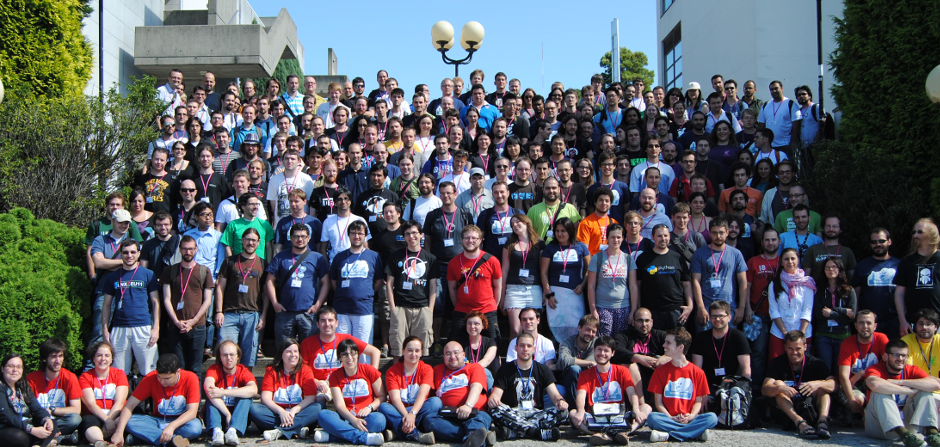
\includegraphics[width=\textwidth]{img/guadec_2012.png}
    \caption{GUADEC A Coruña 2012}
    \label{fig:guadec2012}
\end{figure}

Como comunidade reúne a gran cantidade de persoas tanto voluntarias como profesionais axudaron e axudan a que o proxecto siga adiante. Dentro desta comunidade poden encontrarse persoas de moi diversa procedencia e oficio sendo a maioría programadores aínda que tamén existen persoas dedicadas a marketing, administración, deseño, administración de sistemas, entre outras.

GNOME ademais pon especial interés en intentar sumar xente ao proxecto participando sempre no programa de iniciación ao desenvolvemento de software libre Summer of Code promovido por Google e sendo promotor da iniciativa Outreachy\footnote{Inicialmente denominábase GNOME Outreach Program for Women} que pretende acercar as mulleres á contribución en software libre.

En Europa a comunidade de GNOME reunese na GUADEC, que é o acrónimo de \textbf{G}NOME \textbf{U}sers \textbf{A}nd \textbf{D}evelopers \textbf{C}onference. Un evento que se fai anualmente e que no ano 2012 tivo lugar na Facultade de Informatica da Coruña.

\subsection{Localización e Internacionalización no Proxecto GNOME}
Como xa dixemos un dos aspectos máis importante para o proxecto GNOME é o acercamento as persoas e para lograr isto ponse pleno interés na internacionalización e na localización do ambiente de escritorio e das aplicacións de GNOME. GNOME está traducido a máis de 50 idiomas moitos dos cales teñen máis do 90\% das cadeas traducidas.

O proxecto GNOME emprega o sistema GNU Gettext para internacionalizar e localizar os seus programas e conta con unha plataforma web de nome Damned Lies para xestionar a localización de todo o proxecto. Este programa amosa as estatísticas do estado actual das traducións e axuda a xestionar o ciclo de traballo dos tradutores. Permite asignar módulos a tradutores, que os tradutores suban os ficheiros traducidos e que se faga unha revisión do traballo do tradutor.

Outros proxectos de software como Facebook, Twitter ou, dentro do software libre, Ubuntu e Fedora contan con plataformas online dende as que se pode facer directamente a tradución. GNOME opta por facer a tradución \emph{offline} para que esta sexa dunha maior calidade.

Para que os tradutores poidan traballar de forma cómoda é necesario a existencia de ferramentas que lle faciliten o traballo. Estas ferramentas coñécense como CAT, que é o acrónimo de Computer Assisted Translation. Neste traballo preténdese realizar unha destas ferramentas centrada no proxecto GNOME.

\section{Google Summer of Code}
O Summer of Code, xeralmente abreviado SoC ou GSoC, é un programa da empresa estadounidense Google para o fomento do desarrollo de software libre entre estudientes de todo o mundo. Realizase unha vez ao ano durante o verán estaunidense e os participantes deberán ser estudiantes maiores de 18 anos.

Existen diversas organizaciones de software libre que se prensentan para participar no programa e que aportan unha lista de ideas sobre a que os estudiantes que queiran presnetarse ao programa deberán presentar un proxecto do que queren traballar durante o verán. Se os estudantes son elexidos, a organización asignará a cada estudante un ou máis mentores que deberán guiar ao participante a levar a cabo as tarefas asignadas. Existen avaliacións tanto para os estudantes como para os mentores. Se o estudante é avaliado con éxito recibirán 5500 dolares de parte de Google.

Trátase dun programa de máis éxito con 190 organizacións e 1307 estudantes de todo o mundo durante a edición do verán do ano 2014. 

\section{Motivación}
Durante a GUADEC Hispana\footnote{A GUADEC Hispana é a versión para castelanofalantes da GUADEC} 2012 que tivo lugar en A Coruña dentro da GUADEC do mesmo ano, asistín a unha charla impartida por Daniel Mustieles, o coordinador do equipo de tradutores ao castelán do proxecto GNOME. Nesta charla Daniel, resaltaba a necesidade de que o programa actual de asistencia a tradución fose mellorado. GTranslator está escrito en C e emprega unha biblioteca chamada GObject para facer orientación a obxectos dentro de C. Isto fai que achegarse o proxecto sexa complicado para un novato polo que falando con outros desenroladores da plataforma decidiuse que era mellor reescribir o programa noutra linguaxe e ao mesmo tempo arreglar algúns erros que tiña anteriormente o programa. Durante o ano seguinte presentei un proxecto para o Google Summer of Code para escribir un novo programa CAT para a plataforma GNOME. Este programa sería unha re-escritura e re-deseño de GTranslator nunha linguaxe de programación moito máis amigable, Vala.

\section{Estrutura da memoria}

A memoria componse de oito capítulos nos que se expón os pasos que se deron para crear o programa GNOMECAT.

\paragraph*{Capítulo 1. Introdución.}
Este capítulo. Nel intentamos explicar de forma resumida en que consiste este proxecto, as motivacións para levalo a cabo e a estrutura da memoria.

\paragraph*{Capítulo 2. Estado do Arte.}
Explicaranse as tecnoloxías empregadas no ámbito da internacionalización e localización de software en xeral e software libre en particular. Fárase ademais unha analise de diversas ferramentas do mercado.

\paragraph*{Capítulo 3. Fundamentos Tecnolóxicos.}
Enumeraranse as ferramentas e bibliotecas empregadas durante a elaboración deste proxecto.

\paragraph*{Capítulo 4. Metodoloxía}
Detallarase o conxunto de prácticas e métodos seguidos durante a realización do programa e que están inspiradas fundamentalmente na metodoloxía eXtreme Programming.

\paragraph*{Capítulo 5. Planificación e Seguimento.}
Explicarase a planificación e o seguimento de cada unha das iteracións que fixemos para elaborar o programa.

\paragraph*{Capítulo 6. Análise de Requisitos.}
Explicarase como se levou a cabo o analise de requisitos para esta aplicación e detallarase cada un dos mesmos.

\paragraph*{Capítulo 7. Deseño e implementación.}
Neste capítulo exlicaremos detalles concretos do deseño e a implementación de certas partes do programa.

\paragraph*{Capítulo 8. Conclusións e Traballo Futuro.}
Relataranse as conclusións despois da elaboración do presente proxecto e explicaranse posibles líneas de traballo futuro.





